% Created 2021-09-12 Sun 22:50
% Intended LaTeX compiler: xelatex
\documentclass[letterpaper]{article}
\usepackage{graphicx}
\usepackage{grffile}
\usepackage{longtable}
\usepackage{wrapfig}
\usepackage{rotating}
\usepackage[normalem]{ulem}
\usepackage{amsmath}
\usepackage{textcomp}
\usepackage{amssymb}
\usepackage{capt-of}
\usepackage{hyperref}
\usepackage[margin=1in]{geometry}
\usepackage{fontspec}
\usepackage{indentfirst}
\setmainfont[ItalicFont = LiberationSans-Italic, BoldFont = LiberationSans-Bold, BoldItalicFont = LiberationSans-BoldItalic]{LiberationSans}
\newfontfamily\NHLight[ItalicFont = LiberationSansNarrow-Italic, BoldFont       = LiberationSansNarrow-Bold, BoldItalicFont = LiberationSansNarrow-BoldItalic]{LiberationSansNarrow}
\newcommand\textrmlf[1]{{\NHLight#1}}
\newcommand\textitlf[1]{{\NHLight\itshape#1}}
\let\textbflf\textrm
\newcommand\textulf[1]{{\NHLight\bfseries#1}}
\newcommand\textuitlf[1]{{\NHLight\bfseries\itshape#1}}
\usepackage{fancyhdr}
\pagestyle{fancy}
\usepackage{titlesec}
\usepackage{titling}
\makeatletter
\lhead{\textbf{\@title}}
\makeatother
\rhead{\textrmlf{Compiled} \today}
\lfoot{\theauthor\ \textbullet \ \textbf{2021-2022}}
\cfoot{}
\rfoot{\textrmlf{Page} \thepage}
\titleformat{\section} {\Large} {\textrmlf{\thesection} {|}} {0.3em} {\textbf}
\titleformat{\subsection} {\large} {\textrmlf{\thesubsection} {|}} {0.2em} {\textbf}
\titleformat{\subsubsection} {\large} {\textrmlf{\thesubsubsection} {|}} {0.1em} {\textbf}
\setlength{\parskip}{0.45em}
\renewcommand\maketitle{}
\author{Exr0nZachary Sayyah}
\date{\today}
\title{HW 1\textsubscript{4}}
\hypersetup{
 pdfauthor={Exr0nZachary Sayyah},
 pdftitle={HW 1\textsubscript{4}},
 pdfkeywords={},
 pdfsubject={},
 pdfcreator={Emacs 28.0.50 (Org mode 9.4.4)}, 
 pdflang={English}}
\begin{document}

\maketitle


\section{Limit Laws}
\label{sec:orgf89596f}
see \href{KBe20math401srcLimitLawsBrainstorm.pdf}{pdf}

\section{Openstax Calculus Vol1 2.3 Exercises}
\label{sec:org8bebfc8}
\begin{itemize}
\item \href{https://openstax.org/books/calculus-volume-1/pages/2-3-the-limit-laws}{\textbf{Link}}
\end{itemize}

\subsection{84}
\label{sec:orgf0f3bd1}
\[
\lim_{x\to 1}\frac{x^3+3x^2+5}{4-7x} = \frac{1+3+5}{4-7} = \frac{9}{-3} = \boxed{-3}
\]

\subsection{85}
\label{sec:org1b367c6}
\[
\lim_{x\to -2}\sqrt{x^2-6x+3} = \sqrt{4 - (-12) + 3} = \boxed{\sqrt{19}}
\]

\subsection{86}
\label{sec:org8be6481}
\[
\lim_{x\to_1}\left(9x+1\right)^2 = \left(-9+1\right)^2 = \boxed{64}
\]

\subsection{94}
\label{sec:org1b000c6}
$\backslash$[
\begin{aligned}
\lim_{x\to 4}\frac{x^2-16}{x-4} &= \frac{0}{4-4} = \frac{0}{0}\\
&\Rightarrow \lim_{x\to 2}\frac{\cancel{x-2}}{x\cancel{\left(x-2\right)}} = \lim_{x\to 2}\frac{1}{x} = \boxed{\frac{1}{2}}
\end{aligned}
$\backslash$]

\subsection{98}
\label{sec:orgaf85a50}
\[
\lim_{h\to 0}\frac{\frac{1}{a+h}-\frac{1}{a}}{h} \Rightarrow \frac{ \lim_{h\to 0}\frac{1}{a+h}-\lim_{h\to 0}\frac{1}{a} }{\lim_{h\to 0}h}
\]

now what..?

This is just the derivative of \(\frac{1}{a}\) where \(a\) is a real
valued, non zero constant. So, it should just be
\(\boxed{\frac{-1}{a^2}}\).

\subsubsection{In class review}
\label{sec:org07f2c53}
\[\lim_{h\to 0}\frac{\frac{a-a-h}{(a+h)a}}{h} \Rightarrow \lim_{h\to 0}\frac{-1}{a(a+h)}\]

\subsection{100}
\label{sec:org460df8b}
\[
\lim_{x\to1}\frac{x^3-1}{x^2-1} \Rightarrow \lim_{x\to 1}\frac{\cancel{(x-1)}(x^2+1+x)}{(x+1)\cancel{(x-1)}} = \lim_{x\to 1}\frac{x^2+x+1}{x+1} = \boxed{\frac{3}{2}}
\]

\subsection{Time Check}
\label{sec:orgc5a133e}
It's been an 45 minutes. I will now give up on LaTeXing things:

\begin{center}
\begin{tabular}{rr}
Problem & Result\\
\hline
108 & 2\\
109 & 7\\
110 & 108\\
111 & \(\sqrt{5}\)\\
112 & 36\\
113 & 28\\
114 & 30\\
\end{tabular}
\end{center}

\subsection{116}
\label{sec:orgc3db348}
\begin{center}
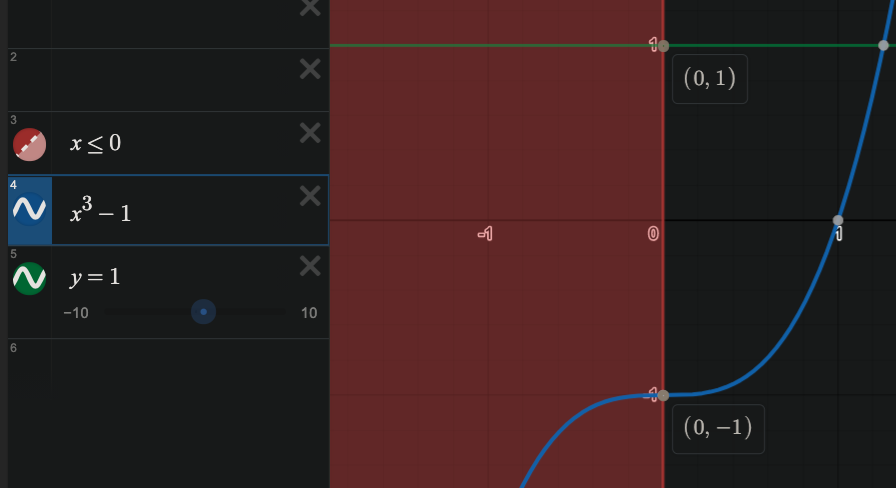
\includegraphics[width=.9\linewidth]{KBe20math401src1u4p116graph.png}
\end{center}

\(\boxed{-1, 1}\)

\subsection{Continuity}
\label{sec:org9466bd7}
\begin{itemize}
\item Function compositions are continuous if their parts are continuous
\item Sum, difference, multiples, powers are continuous if you don't divide
by zero or take an even root of a negative
\end{itemize}

\noindent\rule{\textwidth}{0.5pt}
\end{document}
